\documentclass{article}
\usepackage{amsthm,amssymb,amsmath,multirow,multicol,booktabs}
\usepackage[shortlabels]{enumitem}
\usepackage[utf8]{inputenc}
\usepackage[english]{babel}
\usepackage{tikz}
\usepackage{fancyhdr}

\usetikzlibrary{trees}
\usetikzlibrary{arrows.meta} % <--- Add this line!

\pagestyle{fancy}

\newtheorem*{problem*}{Problem}
\newtheorem*{solution*}{Solution}
\renewcommand{\theenumi}{\alph{enumi}\)}

\title{Dougy's question on money}
\date{7/16/2025}

\begin{document}
\maketitle

\begin{problem*}
    Doug asked a very interesting question: \textbf{How many coins 
    do we need to carry if we were to be able to pay 
    any denomination from 0 to 99 cents?}\\

    I took the liberty to change his question into something 
    completely different: \textbf{Given we have enough coins of each kind
    (Quarters, Dimes, Nickles, and Pennies) in how many different ways 
    can we represent money from 1 to 100 cents?}\\

    So here we will examine my question, and ignore his.
\end{problem*}

\begin{solution*}
We introduce a function, $C(100, Q, D, N, P)$,
representing the number of such combinations,
using quarters (Q), dimes (D), nickles (N), and pennies (P)\\

We make some simple observations. One is that $C(0,\cdots)=1$: 
There is one combination to pay 0 cents (that is to use no coins!)\\

Also $C(100,Q)=1$ (use 4 quarters), and so on\dots\\

\section{A simple example}
As we begin to dive deeper, we see that $C(5, N, P)=2$, the
two combinations that can be visualized with the table:\\

\begin{tabular}{|c|c|}
    \hline
    N & P \\
    \hline
    0 & 5\\
    \hline
    1 & 0\\
    \hline
\end{tabular}

\newpage
\section{Using only Nickles and Pennies}
The following tables will come in handy later:\\

$C(100, N, P)=21$\\
\begin{tabular}{|c|c|}
    \hline
    N & P \\
    \hline
    0 & 100\\
    \hline
    1 & 95\\
    \hline
    2 & 90\\
    \hline
    \dots & \dots\\
    \hline
    20 & 0\\
    \hline
\end{tabular}\\\\

$C(75, N, P)=16$\\
\begin{tabular}{|c|c|}
    \hline
    N & P \\
    \hline
    0 & 75\\
    \hline
    1 & 70\\
    \hline
    2 & 65\\
    \hline
    \dots & \dots\\
    \hline
    15 & 0\\
    \hline
\end{tabular}\\\\  

$C(50, N, P)=11$\\
\begin{tabular}{|c|c|}
    \hline
    N & P \\
    \hline
    0 & 50\\
    \hline
    1 & 45\\
    \hline
    2 & 40\\
    \hline
    \dots & \dots\\
    \hline
    10 & 0\\
    \hline
\end{tabular}\\\\  

$C(25, N, P)=6$\\
\begin{tabular}{|c|c|}
    \hline
    N & P \\
    \hline
    0 & 25\\
    \hline
    1 & 20\\
    \hline
    2 & 15\\
    \hline
    \dots & \dots\\
    \hline
    5 & 0\\
    \hline
\end{tabular}\\\\  

Finally, $C(0, N, P)=1$\\

\newpage
\section{Introducing the Dime!}
Given the previous explorations with just Nickles 
and Pennies, we can build larger tables using the new 
Dime. Let's start with $C(100, D, N, P)$:\\

\begin{tabular}{|c|c|c|c|}
    \toprule
    D & N & P & Notice\\
    \hline
    \textbf{0} & 0 & 100 & \multirow{5}{*}{{
        $C(100, N, P)=21$ combinations
    }} \\
    \cline{1-3}
    0 & 1 & 95 & \\
    \cline{1-3}
    0 & 2 & 90 & \\
    \cline{1-3}
    0 & \dots & \dots & \\
    \cline{1-3}
    0 & 20 & 0 & \\

    \bottomrule
    \textbf{1} & 0 & 90 & \multirow{3}{*}{{
        $C(90, N, P)$ combinations
    }} \\
    \cline{1-3}
    1 & 1 & 85 & \\
    \cline{1-3}
    1 & \dots & \dots & \\

    \bottomrule
    \textbf{2} & \multicolumn{3}{|c|}{{$C(80, N, P)$}} \\

    \bottomrule
    \textbf{3} & \multicolumn{3}{|c|}{{$C(70, N, P)$}} \\

    \bottomrule
    \textbf{\dots} & \multicolumn{3}{|c|}{{\dots}} \\

    \bottomrule
    \textbf{10} & \multicolumn{3}{|c|}{{$$C(0, N, P)=1$$}} \\

    \bottomrule
\end{tabular}\\\\

Hence we that $C(100, D, N, P)$ depends on various 
$C(100, N, P)$, $C(90, N, P)$, etc.
Similarly, it's easy to see that:\\

\begin{tabular}{|c|c|c|c|}
    \hline
    Q & D & N & P \\
    \bottomrule
    \textbf{0} & \multicolumn{3}{|c|}{{$$C(100, D, N, P)$$}} \\

    \bottomrule
    \textbf{1} & \multicolumn{3}{|c|}{{$$C(75, D, N, P)$$}} \\

    \bottomrule
    \textbf{2} & \multicolumn{3}{|c|}{{$$C(50, D, N, P)$$}} \\

    \bottomrule
    \textbf{3} & \multicolumn{3}{|c|}{{$$C(25, D, N, P)$$}} \\

    \bottomrule
    \textbf{4} & \multicolumn{3}{|c|}{{$$C(0, D, N, P)=1$$}} \\

    \bottomrule
\end{tabular}\\\\

\newpage
\section{Trees with Dimes, Nickles, \& Pennies}

\begin{figure}[htbp]
\centering
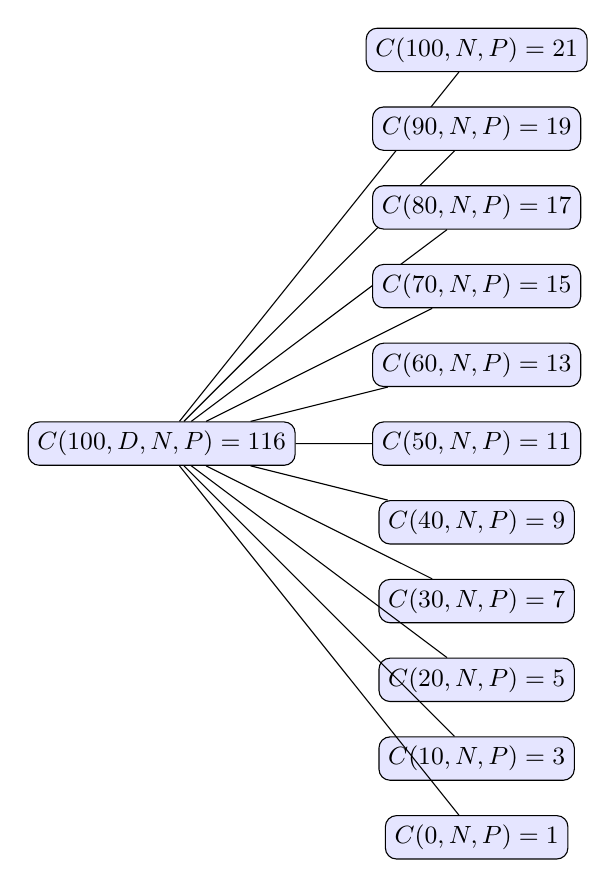
\begin{tikzpicture}[
    grow'=right, % This makes the tree grow from left to right (sideways)
    level distance=4cm, % Distance between levels (horizontal distance)
    sibling distance=1cm, % Distance between sibling nodes (vertical distance)
    every node/.style={
        draw, % Draw a border around nodes
        rounded corners, % Rounded corners for nodes
        fill=blue!10, % Light blue fill color
        align=center, % Center text within nodes
        font=\sffamily\small % Sans-serif font, small size
    },
    % edge from parent/.style={draw, -Latex'} % Style for the connecting lines (arrows)
]

\node {$C(100,D,N,P)=116$}
    child { node {$C(100,N,P)=21$} }
    child { node {$C(90,N,P)=19$} }
    child { node {$C(80,N,P)=17$} }
    child { node {$C(70,N,P)=15$} }
    child { node {$C(60,N,P)=13$} }
    child { node {$C(50,N,P)=11$} }
    child { node {$C(40,N,P)=9$} }
    child { node {$C(30,N,P)=7$} }
    child { node {$C(20,N,P)=5$} }
    child { node {$C(10,N,P)=3$} }
    child { node {$C(0,N,P)=1$} }
;
\end{tikzpicture}

\caption{116 conbinations (100 cents using D, N, and P)}
\label{fig:sideways_tree} % Label for cross-referencing
\end{figure}

\begin{figure}[htbp]
\centering

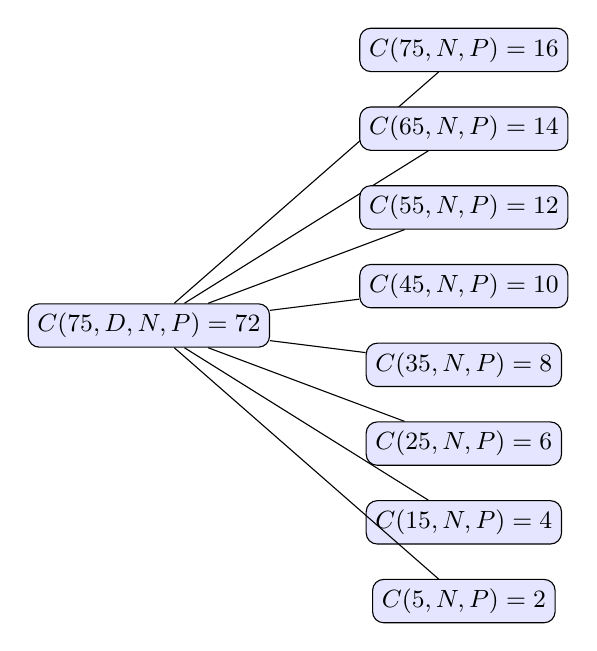
\begin{tikzpicture}[
    grow'=right, % This makes the tree grow from left to right (sideways)
    level distance=4cm, % Distance between levels (horizontal distance)
    sibling distance=1cm, % Distance between sibling nodes (vertical distance)
    every node/.style={
        draw, % Draw a border around nodes
        rounded corners, % Rounded corners for nodes
        fill=blue!10, % Light blue fill color
        align=center, % Center text within nodes
        font=\sffamily\small % Sans-serif font, small size
    },
    % edge from parent/.style={draw, -Latex'} % Style for the connecting lines (arrows)
]

\node {$C(75,D,N,P)=72$}
    child { node {$C(75,N,P)=16$} }
    child { node {$C(65,N,P)=14$} }
    child { node {$C(55,N,P)=12$} }
    child { node {$C(45,N,P)=10$} }
    child { node {$C(35,N,P)=8$} }
    child { node {$C(25,N,P)=6$} }
    child { node {$C(15,N,P)=4$} }
    child { node {$C(5,N,P)=2$} }
;
\end{tikzpicture}

\caption{72 combinations (75 cents using D, N, and P)}
\label{fig:sideways_tree} % Label for cross-referencing
\end{figure}

\begin{figure}[htbp]
\centering

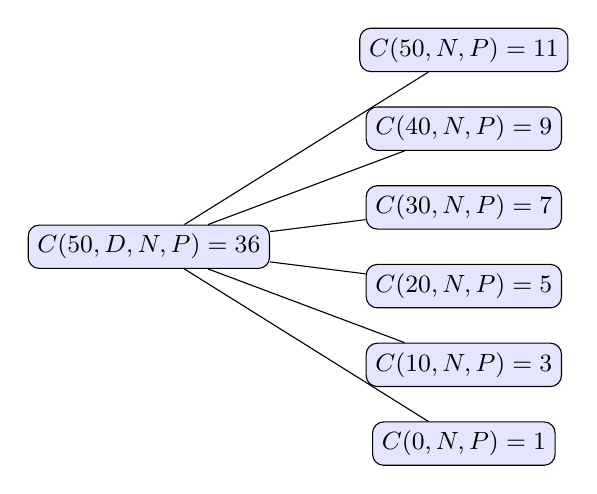
\begin{tikzpicture}[
    grow'=right, % This makes the tree grow from left to right (sideways)
    level distance=4cm, % Distance between levels (horizontal distance)
    sibling distance=1cm, % Distance between sibling nodes (vertical distance)
    every node/.style={
        draw, % Draw a border around nodes
        rounded corners, % Rounded corners for nodes
        fill=blue!10, % Light blue fill color
        align=center, % Center text within nodes
        font=\sffamily\small % Sans-serif font, small size
    },
    % edge from parent/.style={draw, -Latex'} % Style for the connecting lines (arrows)
]

\node {$C(50,D,N,P)=36$}
    child { node {$C(50,N,P)=11$} }
    child { node {$C(40,N,P)=9$} }
    child { node {$C(30,N,P)=7$} }
    child { node {$C(20,N,P)=5$} }
    child { node {$C(10,N,P)=3$} }
    child { node {$C(0,N,P)=1$} }
;
\end{tikzpicture}

\caption{36 combinations (50 cents using D, N, and P)}
\label{fig:sideways_tree} % Label for cross-referencing
\end{figure}

\begin{figure}[htbp]
\centering

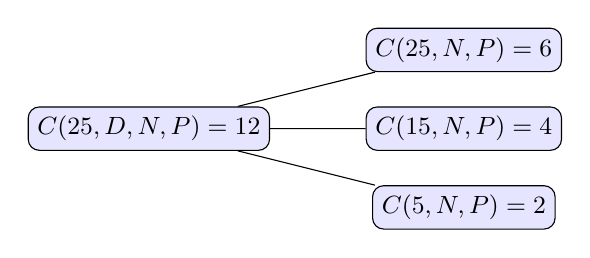
\begin{tikzpicture}[
    grow'=right, % This makes the tree grow from left to right (sideways)
    level distance=4cm, % Distance between levels (horizontal distance)
    sibling distance=1cm, % Distance between sibling nodes (vertical distance)
    every node/.style={
        draw, % Draw a border around nodes
        rounded corners, % Rounded corners for nodes
        fill=blue!10, % Light blue fill color
        align=center, % Center text within nodes
        font=\sffamily\small % Sans-serif font, small size
    },
    % edge from parent/.style={draw, -Latex'} % Style for the connecting lines (arrows)
]

\node {$C(25,D,N,P)=12$}
    child { node {$C(25,N,P)=6$} }
    child { node {$C(15,N,P)=4$} }
    child { node {$C(5,N,P)=2$} }
;
\end{tikzpicture}

\caption{12 combinations (25 cents using D, N, and P)}
\label{fig:sideways_tree} % Label for cross-referencing
\end{figure}

\newpage
\section{Putting it all together}

The last coin, the Quarter,
can be used 0, 1, 2, 3, or 4 times. 
The following tree shows the desired root node, 
and its dependency on the five previously established values:\\

\begin{figure}[htbp]
\centering
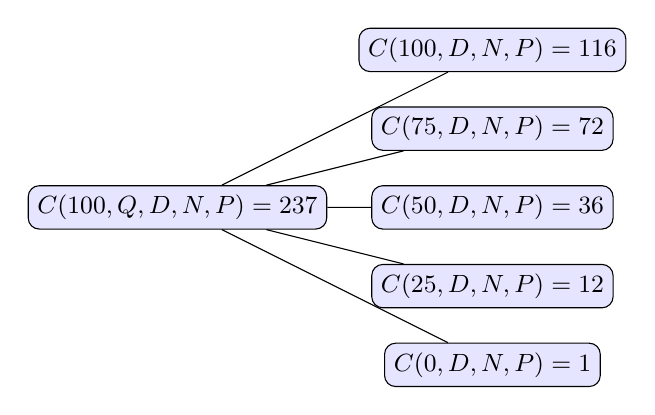
\begin{tikzpicture}[
    grow'=right, % This makes the tree grow from left to right (sideways)
    level distance=4cm, % Distance between levels (horizontal distance)
    sibling distance=1cm, % Distance between sibling nodes (vertical distance)
    every node/.style={
        draw, % Draw a border around nodes
        rounded corners, % Rounded corners for nodes
        fill=blue!10, % Light blue fill color
        align=center, % Center text within nodes
        font=\sffamily\small % Sans-serif font, small size
    },
    % edge from parent/.style={draw, -Latex'} % Style for the connecting lines (arrows)
]

\node {$C(100,Q,D,N,P)=237$} % The root of the tree
    child { node {$C(100,D,N,P)=116$} }
    child { node {$C(75,D,N,P)=72$} }
    child { node {$C(50,D,N,P)=36$} }
    child { node {$C(25,D,N,P)=12$} }
    child { node {$C(0,D,N,P)=1$} }
    ;
\end{tikzpicture}

\caption{277 combinations (100 cents using Q, D, N, and P)}
\label{fig:sideways_tree} % Label for cross-referencing
\end{figure}

Thus we see that using all four kind of coins,
we have $237$ combinations to represent any value 
from 0 to 100 cents.

\end{solution*}

\end{document}
